NetVis is a Java application which uses OpenGL to draw visualizations and Swing to provide a graphical user interface for displaying further information and allowing the user to customise the visualizations.

In designing the application, we have focused on maintaining extensibility and keeping a modular programming style. It is simple to add support for additional input data formats, or to develop a new visualization that utilises the same data processing engine.

Packet data is transferred to the application as a CSV packet capture file. NetVis uses a file format that can be directly obtained from the packet analyser Wireshark and other similar applications. NetVis will process each packet and analyse its fields which includes a time stamp, information about the packet's source (IP, hardware (MAC) address, port), information about the packet's destination, communication protocol, and the packet length in bytes.
The current version of NetVis does not process the content of packets.

A convenient feature of the data input system is a time control system. The CSV file is processed as if its packets would arrise in a live network. The user can choose to speed up or slow down the speed with which packets are fed into the application, can pause processing, or skip towards the end of the data record. This is helpful in analysing the data since critical time intervals can be analysed in more detail.

The application is set up in such a way that it is also easy to use the activity of a live network as its input source.

The input data is processed in a data controller which supplies the visualizations and the user interface with packet data. If the user has chosen to apply filters to the data, the data controller only directs the filtered data stream to the rest of the application, so that all parts share a common data source.

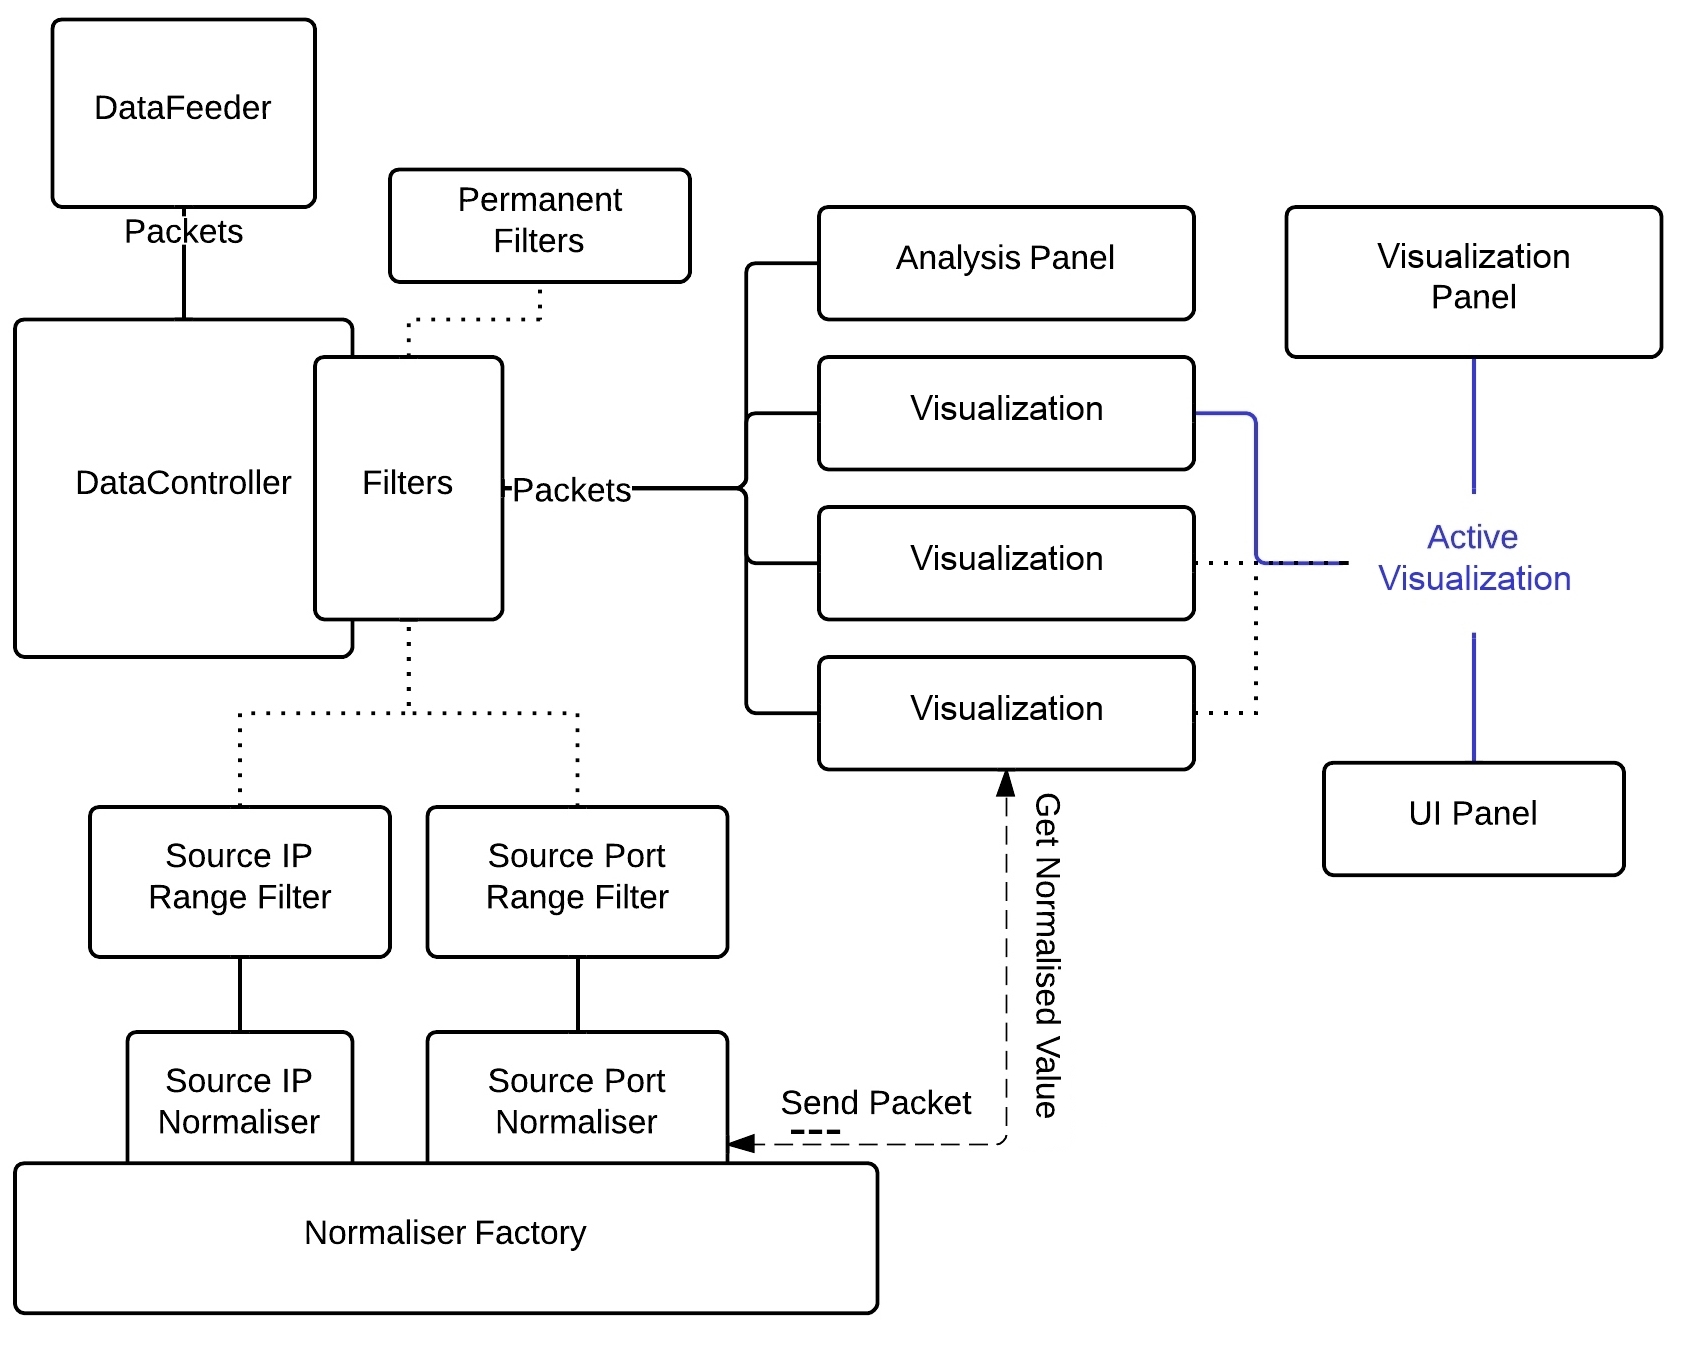
\includegraphics[width=\linewidth]{materials/architecture.jpg}

NetVis includes a data filtering system that allows users to select a subset of processed packets which exhibit features which the user specified to be of interest.

The application supports two types of filters: filters that the user explicitly defines, and filters applied on-the-fly from within the visualizations.
Both types are applied to all visualizations and information displayed, and they can be adjusted at any time without losing prior data.

There are a variety of filter controls.  First, there is a menu for filtering by transit protocol. By default, all protocols are selected and therefore included. Protocols are sorted into menus by protocol family, appearing in multiple places where appropriate. Second, there is a control to select the range of ports the application uses, which defaults to the maximum port range.  The source and destination ports can be set separately, enabling a user to view all data entering/exiting a port as desired.  Third, there are IP and MAC address filters.  These work on a blacklist/whitelist system, allowing a user to only view packets to or from a particular set of addresses, or to ignore packets going to or from a different set.  This enables a user to, for instance, ignore traffic from sources they know are irrelevant or focus only on an address that is causing concern.

The packet attributes that are processed by NetVis do not share a common scale, nor are they necessarily orderable. It is, however, desirable to map some of these properties into a shared representation which allows a more intuitive grasp of the distribution of attributes. We achieve this by processing the packets in a `normalising' system. This system keeps track of the used values and maps them into the interval $[0,1]$. In this way all normalised packets can be displayed in relation to a number axis. This representation is used in three different visualizations.

Each normaliser is able to create a temporary filter in the application that will filter its corresponding attribute on a certain range.
Since the normalising class is in control of its filter this creates a zooming effect based on the range of the filter: the lower bound is normalised to 0, the upper bound to 1. 


%Modularity: \textbf{[Make this better.]}
%The application was designed to be very extensible.  Adding a new visualization is simply a matter of adding it to the application's list of those available, which will cause it to be included and kept up-to-date as packets come in and are filtered.  The same is true for filters and normalisers.  \textbf{[wrong place:] }Adding a filter would result in its controls automatically being included in the right panel and all packets would then be filtered according to the criteria it specifies.  Adding a normaliser would cause it to be integrated with the Spinning Cube, Dataflow and Attribute Distribution visualizations.  This modularity extends even so far as data input.  If a class were written to accept packets from a different source, it would be trivial to switch the application to use this class.